\documentclass[10pt,a4paper]{article}

% ─── Packages ─────────────────────────────────────────

\usepackage{fontspec}
\setmainfont{Times New Roman}

\usepackage[top=0.6cm,bottom=0.5cm,left=1.45cm,right=1.45cm]{geometry}

\usepackage{titlesec}
\usepackage{enumitem}
\usepackage{hyperref}
\usepackage{xcolor}
\usepackage{tabularx}
\usepackage{graphicx}
\usepackage{parskip}

% ─── Colors ───────────────────────────────────────────

\definecolor{primary}{RGB}{30,40,90}
\definecolor{namecolor}{RGB}{0,120,180}
\definecolor{accent}{RGB}{50,90,150}
\definecolor{rulecol}{RGB}{200,205,220}
\definecolor{gray}{RGB}{90,90,90}

\hypersetup{
    colorlinks=true,
    urlcolor=accent
}

\pagestyle{empty}
\setlength{\parskip}{0pt}

% ─── Section ──────────────────────────────────────────

\titleformat{\section}
    {\normalsize\bfseries\color{primary}}
    {}
    {0em}
    {}
    [\vspace{1pt}\textcolor{rulecol}{\titlerule[0.6pt]}\vspace{1pt}]

\titlespacing{\section}{0pt}{3pt}{1pt}

% ─── Entry ────────────────────────────────────────────

\newcommand{\entry}[3]{%
    \noindent
    \begin{tabularx}{\linewidth}{X r}
        \textbf{\color{primary}#1} &
        {\scriptsize\color{gray}#2}
    \end{tabularx}\\[-2pt]
    {\scriptsize\textit{\color{gray}#3}}
    \vspace{0.5pt}
}

% ─── Compact list ─────────────────────────────────────

\newenvironment{cvitems}{
    \begin{itemize}[
        leftmargin=1.1em,
        topsep=0pt,
        itemsep=0.3pt,
        parsep=0pt,
        partopsep=0pt
    ]
}{
    \end{itemize}
}

% ═════════════════════════════════════════════════════

\begin{document}

% ─── HEADER ───────────────────────────────────────────

\noindent

\begin{tabularx}{\linewidth}{@{}X r@{}}

\begin{minipage}[c]{\linewidth}

    {\LARGE\bfseries\color{namecolor} Ho Huynh Nhu}\\[1pt]

    {\large\bfseries\color{primary}
    Business Analyst Assistant}\\[2pt]

    {\scriptsize\color{gray}
    20/10/2003
    \enspace\textcolor{rulecol}{|}
    \enspace (+84) 367 503 477
    \enspace\textcolor{rulecol}{|}
    \enspace
    \href{mailto:hhnhu2003@gmail.com}{hhnhu2003@gmail.com}
    \enspace\textcolor{rulecol}{|}
    \enspace Ho Chi Minh City}\\[1pt]

    {\scriptsize
    \href{https://github.com/hohuynhnhu}
    {github.com/hohuynhnhu}
    \enspace\textcolor{rulecol}{|}
    \enspace
    \href{https://www.facebook.com/huynhnhu.ho.961}
    {facebook.com/huynhnhu.ho.961}
    }

\end{minipage}

&

\begin{minipage}[c]{2.1cm}
    \raggedleft
    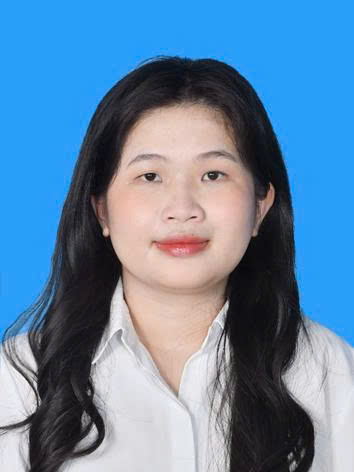
\includegraphics[
        width=2.1cm,
        height=2.5cm,
        keepaspectratio
    ]{assets/avt.jpg}
\end{minipage}

\end{tabularx}

\vspace{1pt}

\textcolor{rulecol}{\rule{\linewidth}{0.6pt}}

% ─── CAREER OBJECTIVE ─────────────────────────────────

\section*{Career Objective}

{\small
Final-year Information Technology student seeking a Business Analyst Assistant
position. Experienced in cleaning, validating, and analyzing data, building
reports and dashboards, and programming in Python, SQL, and JavaScript.
Careful, honest, and proactive, with strong logical thinking and a focus on
data accuracy. Eager to support the data and project reporting team, learn
research data tools such as SPSS, and communicate findings clearly to
managers and related departments.
}

% ─── EDUCATION ────────────────────────────────────────

\section*{Education}

\entry
{University of Transport Ho Chi Minh City (UTH)}
{10/2022 -- 10/2026}
{Bachelor of Information Technology -- Completed coursework}

{\small
\begin{cvitems}

    \item GPA: \textbf{3.4 / 4.0}

    \item \textbf{Excellent Scholarship} -- Semester 1, 2025

    \item \textbf{Second Prize -- AI Track},
    UTH Student Scientific Research Conference 2025

\end{cvitems}
}

% ─── SKILLS ───────────────────────────────────────────

\section*{Skills}

{\small

\begin{tabularx}{\linewidth}{@{}lX@{}}

\textbf{Data Analysis}
&
Data Cleaning, Data Validation \& Accuracy Checking, Exploratory Data Analysis (EDA),
Trend Analysis, KPI Analysis, Statistical Analysis
\\[1pt]

\textbf{Programming}
&
Python (Pandas, NumPy), SQL, JavaScript, TypeScript
\\[1pt]

\textbf{SQL / Databases}
&
PostgreSQL, SQL Server, MySQL, Joins, CTEs, Aggregations,
Subqueries, Window Functions
\\[1pt]

\textbf{Excel}
&
Pivot Table, Lookup Functions, Data Cleaning, Filtering, Reporting
\\[1pt]

\textbf{BI / Visualization}
&
Power BI, DAX, Dashboard Development, Data Visualization,
Matplotlib, Seaborn
\\[1pt]

\textbf{ETL / Automation}
&
ETL/ELT, dbt, Apache Airflow, Data Pipeline
\\[1pt]

\textbf{Tools \& Collaboration}
&
Jira, Confluence, Git, Docker, Postman, VS Code

\end{tabularx}

}

% ─── WORK EXPERIENCE ──────────────────────────────────

\section*{Work Experience}

\entry
{Gotik Consulting -- Data Engineer}
{Python \textbar{} dbt \textbar{} PostgreSQL \textbar{} Airflow \textbar{} Power BI}
{03/2026 -- 05/2026}

{\small
\begin{cvitems}
    \item Cleaned, checked, and standardized Odoo business data with Python and SQL to detect discrepancies and ensure the accuracy of datasets used for analysis and reporting.

    \item Wrote SQL queries to aggregate, filter, and join data, cross-checking results to provide reliable figures for reports.

    \item Built Power BI dashboards and prepared regular reports on operational metrics to support management decisions.

    \item Developed dbt models and Python ETL pipelines, automated with Apache Airflow, to turn raw data into structured, reusable analytical datasets.
\end{cvitems}
}

% ─── PROJECTS ─────────────────────────────────────────

\section*{Featured Projects}

\entry
{Delivery Driver -- Order Analytics System}
{Python \textbar{} SQL \textbar{} Kafka \textbar{} PostgreSQL \textbar{} Power BI}
{12/2025 -- 02/2026}

{\small
\begin{cvitems}
    \item Built an automated data pipeline with a Data Lake and Data Warehouse to collect, process, and prepare order data for analysis.
    \item Applied RFM and Association Rule Mining to analyze customer behavior and frequent pickup--delivery location patterns, generating insights for business recommendations.
    \item GitHub: \href{https://github.com/LeKhang-cn22h/BE-delivery-driver}{BE-delivery-driver}
\end{cvitems}
}

\vspace{1pt}

\entry
{VehicleScan -- Smart Parking Data System}
{Python \textbar{} SQL \textbar{} PostgreSQL \textbar{} Firebase \textbar{} ESP32}
{03/2025 -- 03/2026}

{\small
\begin{cvitems}
    \item Collected and processed vehicle and IoT sensor data with Python and SQL for real-time parking management.
    \item Integrated AI, sensor, and application data into one centralized system to support monitoring and data analysis.
    \item GitHub: \href{https://github.com/LeKhang-cn22h/VehicleScanner}{VehicleScanner}
\end{cvitems}
}

% \vspace{1pt}

% \entry
% {Fall Detection -- Machine Learning Classification System}
% {Python \textbar{} PyTorch \textbar{} YOLOv8 Pose \textbar{} MediaPipe \textbar{} Transformer}
% {04/2026 -- 06/2026}

% {\small
% \begin{cvitems}
%     \item Prepared video datasets and trained a Transformer Encoder for fall/non-fall classification, achieving 97.8\% mean accuracy with 5-fold cross-validation and testing on unseen data.
% \end{cvitems}
% }

% ─── ADDITIONAL INFORMATION ───────────────────────────

\section*{Additional Information}

{\small

\begin{tabularx}{\linewidth}{@{}lX@{}}

\textbf{Soft Skills}
&
Logical thinking \textbar{} Time management and multitasking \textbar{}
Careful, honest, proactive \textbar{} Clear communication

\\[1pt]

\textbf{English}
&
TOEIC 500; technical document reading and basic professional communication

\\[1pt]

\textbf{Availability}
&
Available for full-time Business Analyst Assistant opportunities.

\end{tabularx}

}
\end{document}